%!TEX program = xelatex
\documentclass[10pt,twocolumn,letterpaper]{article}

\usepackage{cvpr}
\usepackage{times}
\usepackage{epsfig}
\usepackage{graphicx}
\usepackage{tabularx}
\usepackage{amsmath}
\usepackage{amssymb}
\usepackage{amsthm}
\usepackage{algorithm2e}
\usepackage{authblk}


% Include other packages here, before hyperref.

% If you comment hyperref and then uncomment it, you should delete
% egpaper.aux before re-running latex.  (Or just hit 'q' on the first latex
% run, let it finish, and you should be clear).
\usepackage[pagebackref=true,breaklinks=true,letterpaper=true,colorlinks,bookmarks=false]{hyperref}

\usepackage{fontspec}

\cvprfinalcopy % *** Uncomment this line for the final submission

\def\cvprPaperID{407} % *** Enter the CVPR Paper ID here
\def\httilde{\mbox{\tt\raisebox{-.5ex}{\symbol{126}}}}

\def\vec{\mathbf}
\def\mat{\mathbf}

\newtheorem{lemma}{Lemma}
\newtheorem{theorem}{Theorem}
\newtheorem{proposition}{Proposition}

% Pages are numbered in submission mode, and unnumbered in camera-ready
\ifcvprfinal\pagestyle{empty}\fi
\begin{document}

\RestyleAlgo{boxruled}

%%%%%%%%% TITLE
\title{Learning From Massive Noisy Labeled Data for Image Classification}

\author[1]{Tong Xiao}
\author[2]{Tian Xia}
\author[2]{Yi Yang}
\author[2]{Chang Huang}
\author[1]{Xiaogang Wang}

\affil[1]{The Chinese University of Hong Kong}
\affil[2]{Baidu Research}

\renewcommand\Authands{ and }

% For a paper whose authors are all at the same institution,
% omit the following lines up until the closing ``}''.
% Additional authors and addresses can be added with ``\and'',
% just like the second author.
% To save space, use either the email address or home page, not both

\maketitle
%\thispagestyle{empty}

%%%%%%%%% ABSTRACT
\begin{abstract}
Large-scale supervised datasets are crucial to train deep neural networks for various computer vision problems. However, obtaining a massive amount of well labeled data is usually very expensive and time consuming. In this paper, we introduce a general framework to train deep nets with only limited number of clean labels and millions of easily obtained noisy labels. We model label noises with a graphical probabilistic framework and further integrate it into the deep learning system. To demonstrate the performance of our approach, we collect a large scale clothing classification dataset with both noisy and clean labels. We demonstrate the effectiveness of our approach on this dataset, showing the possibility of learning a strong deep model with only a small amount of clean labels.
\end{abstract}

%%%%%%%%% BODY TEXT
\section{Introduction} % (fold)
\label{sec:introduction}

Deep learning with massive amount of supervised training data has recently shown very impressive improvement on multiple image recognition challenges including image classification~\cite{krizhevsky2012imagenet}, attribute learning~\cite{zhang2013panda}, scene classification~\cite{farabet2013learning}, etc. While state-of-the-art results have been continuously reported~\cite{zeiler2013visualizing,simonyan2014very,szegedy2014going}, all these methods require reliable annotations from millions of images~\cite{deng2009imagenet} which are often expensive and time-consuming to obtain~\cite{deng2009imagenet}, preventing deep models from being quickly trained on new image recognition problems. Thus it is necessary to develop new efficient labeling and training frameworks for deep learning.

One possible solution is to automatically collect large amount of annotations from the Internet web images~\cite{gong2014multiview} (i.e. extracting tags from the surrounding texts or keywords from search engines) and directly use them as ground truth to train deep models. Unfortunately, these labels are extremely unreliable due to the various types of noise (i.e. labeling mistakes from annotators or computing errors from extraction algorithms). Many works have shown that these noisy labels could adversely impact the classification accuracy of the induced classifiers~\cite{zhu2004class,nettleton2010study,pechenizkiy2006class}. Various noise-robust algorithms are developed but experiments show that performances of classifiers inferred by robust algorithms are still affected by label noise. Other noise cleaning algorithms are developed~\cite{barandela2000decontamination,brodley2011identifying}, but these approaches are difficult in distinguishing informative hard examples from harmful mislabeled ones. 

\begin{figure}[t]
\begin{center}
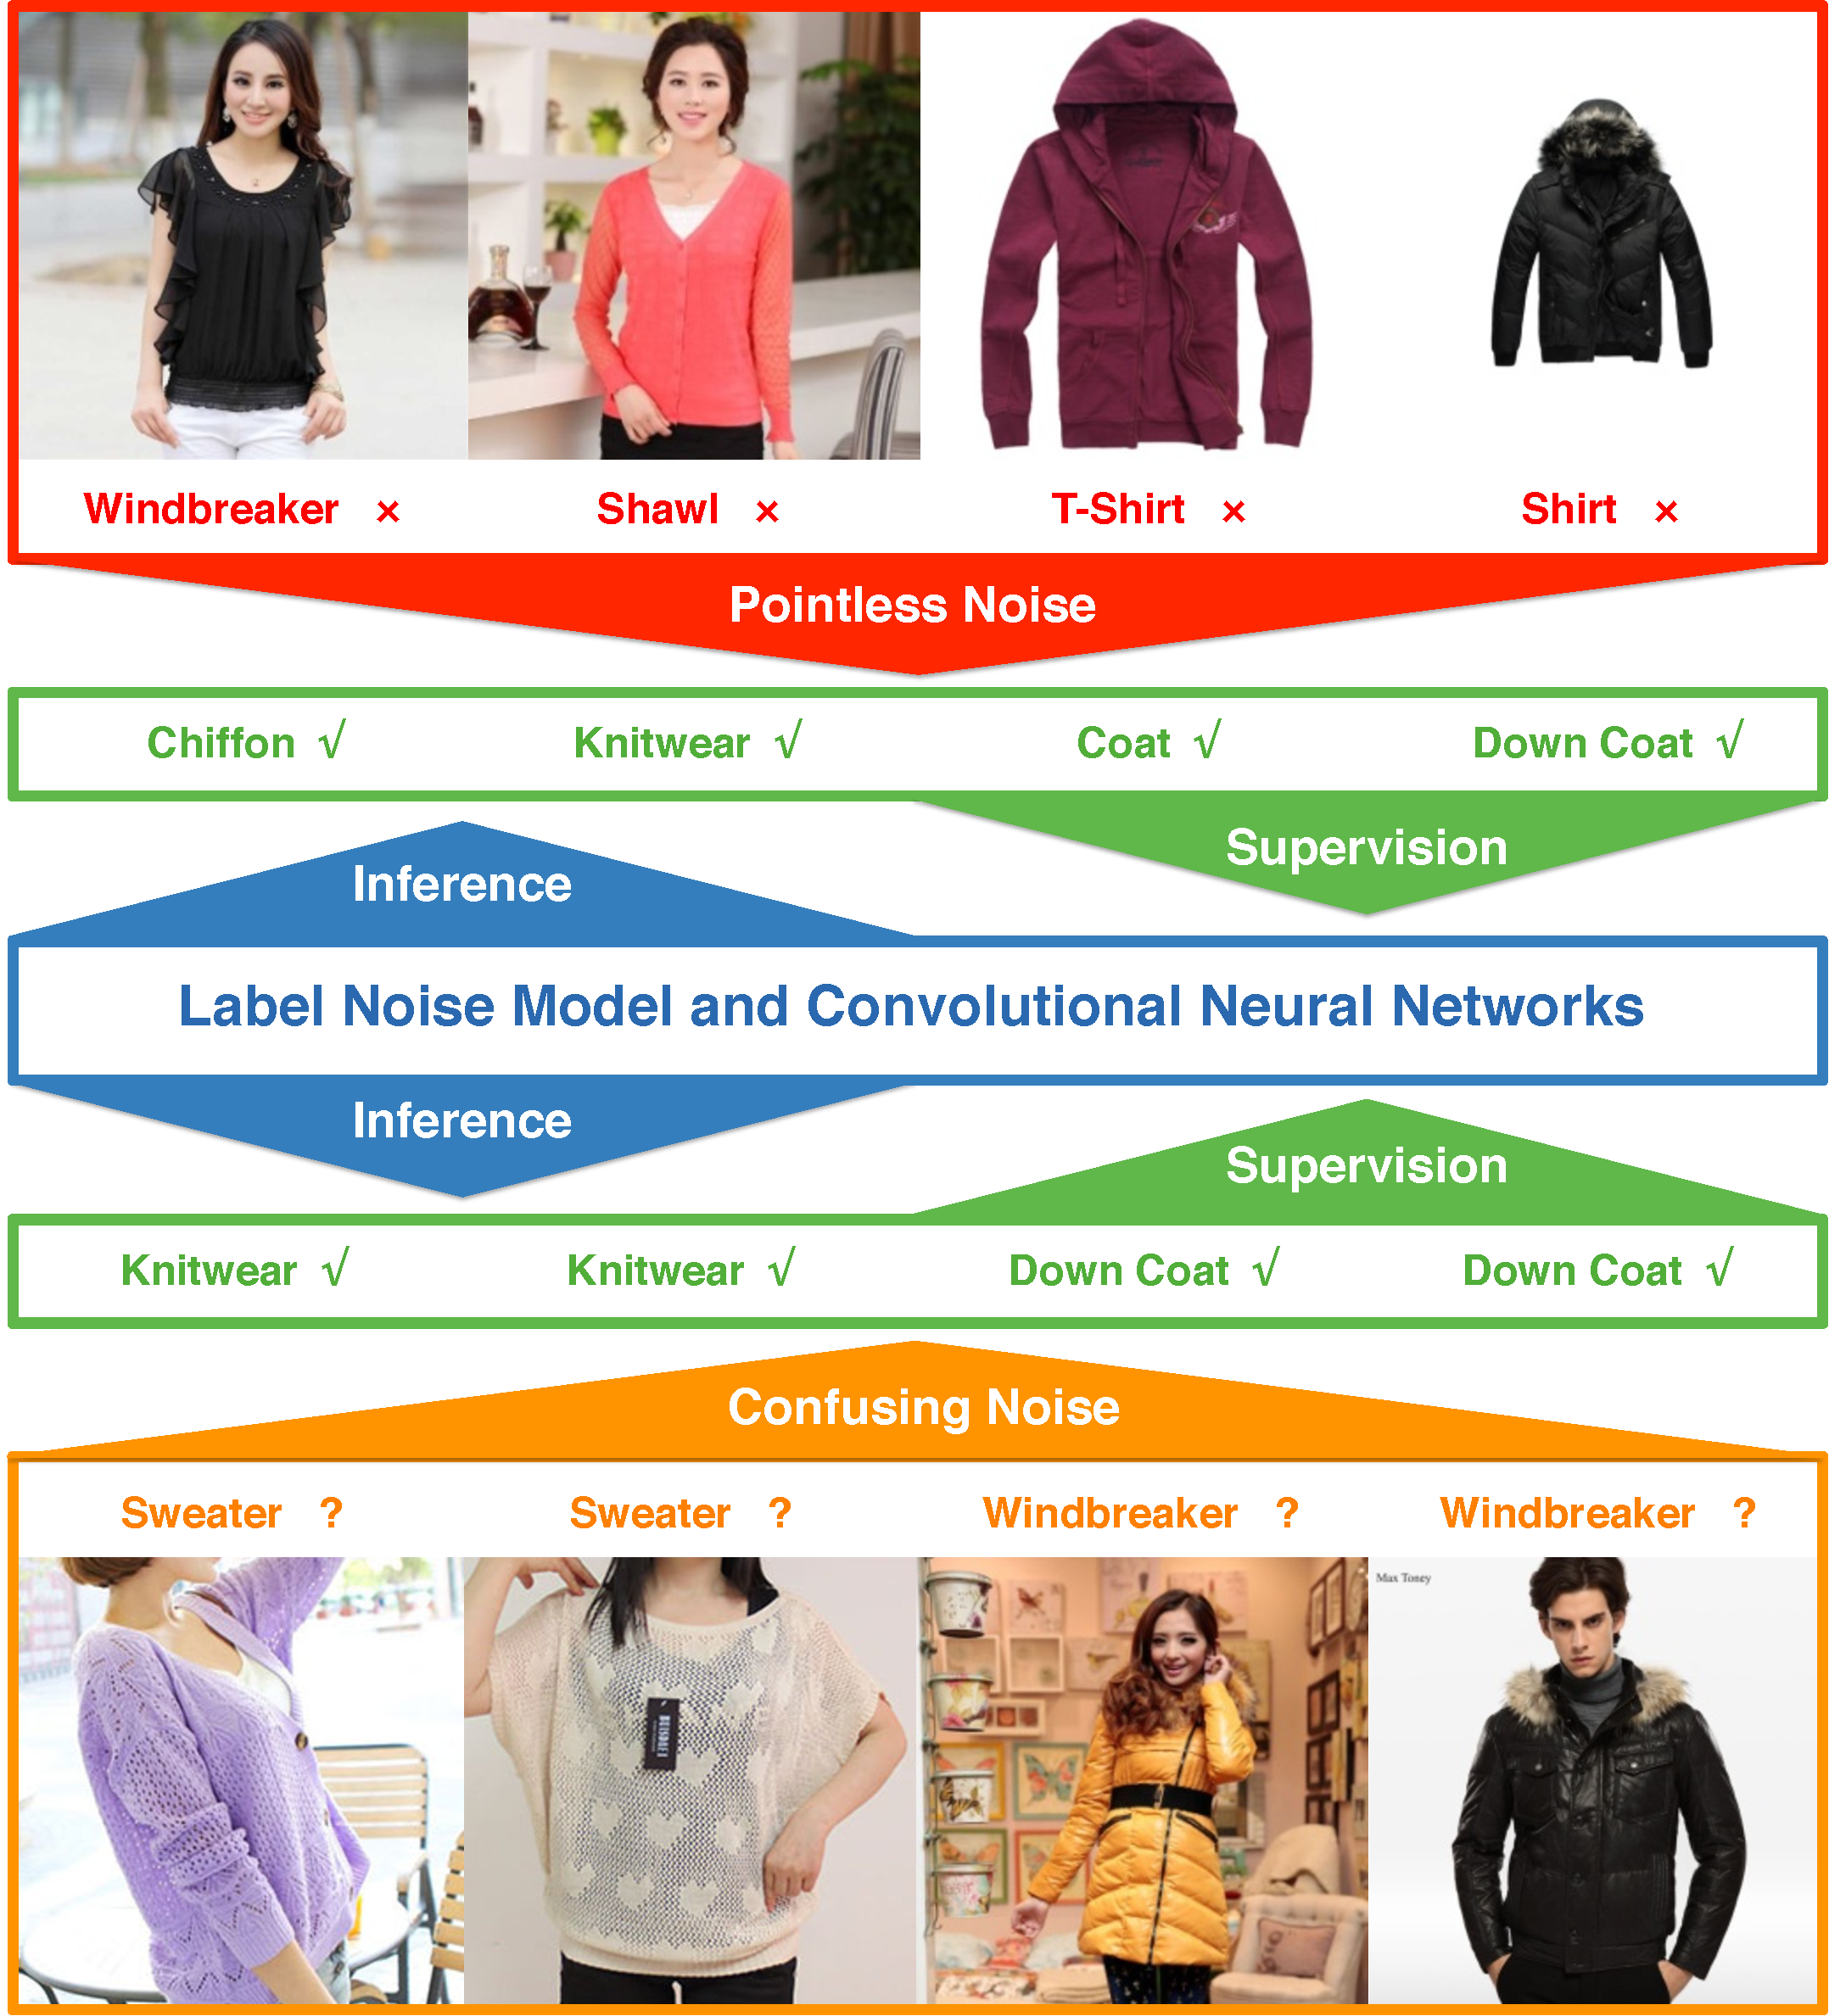
\includegraphics[width=0.9\linewidth]{figure/overview.pdf}
\end{center}
\caption{Overview of our method. Labels of web images often suffer from different types of noise. Our deep model infers true labels based on observed images and noisy labels. These true labels are then used to supervise the training of CNNs.}
\label{fig:overview}
\end{figure}

Although annotating all the noisy data is costly, it is often easy to obtain a small amount of clean labels. Based on the observation of transferability of deep neural networks, people first initialize the parameters with a model pretrained on a larger yet related dataset~\cite{krizhevsky2012imagenet}, and then finetuning on the smaller dataset of specific task~\cite{oquab2013learning,azizpour2014generic}. Such methods may better avoid overfitting and utilize the relationships between the two datasets. However, we find that training a deep model directly with massive noisy data could achieve better performance than finetuning from a pretrained ImageNet model over a small subset, especially when the relations between the two datasets are weak. Other approaches address the classification problem as semi-supervised learning where noisy labels are discarded~\cite{zhu2002learning}. These algorithms usually suffer from model complexity thus cannot be applied on large-scale datasets. 

Our goal here is to build an end-to-end deep learning system that is capable of training with both limited clean labels and massive amount of noisy labels more effectively. Figure~\ref{fig:overview} shows the general framework of our system. The major challenge of using noisy labeled data is to identify bad samples and keep them from drifting the model training. Intuitively, we have two types of evidence to help make decisions. One comes from the ground truth labels of other similar images, and the other comes from how confusing the input image itself. In this paper, we model these two types of information as latent variables and use them to bridge the semantic gap between our observed image and weak label. Additionally, we introduce two types of label noise:
\begin{itemize}
   \item \textbf{Pure random noise} occurs when a noisy label has no semantic relationship with its image, for example, the samples with ``$\times$'' in Figure~\ref{fig:overview}. This kind of noise is often caused by either the mismatch between web image and surrounding texts, or false conversion from text to label. The noisy label in this case is not acceptable.
   \item \textbf{Confusing noise} occurs when a noisy label is a reasonable object class for its image other than the ground truth one. This kind of noise happens regularly in some sort of images. For example, the samples with ``?'' in Figure~\ref{fig:overview}. However, in real applications, confusion among several related labels is generally acceptable to users.
\end{itemize}

We propose a novel probabilistic model to capture the relations among all these factors. We solve the problem by Expectation-Maximization (EM) algorithm and integrate it into a deep learning framework. To validate our approach, we collect a clothing classification dataset consisting of around $72,000$ clean labeled and one million noisy labeled data. Experiments on this dataset demonstrate that massive noisy labeled data could benefit the training of deep neural networks.

Our work is inspired by~\cite{sukhbaatar2014learning}, which also modifies the deep neural networks to train effectively with noisy labeled data. However, their modification is simply implemented by adding a linear layer on top of the softmax layer, which builds on the assumption that label noise is independent with input images. We generalize~\cite{sukhbaatar2014learning} to a new deep learning framework by relating the noise to the input image. We find that by modeling the noise more appropriately, the deep models can benefit even more from noisy labels.

Our contribution comes from three aspects. First, we model label noise generation with a graphical model and further integrate it into the deep learning framework. Second, we study different noise types and model their relations with the images by a deep neural network. Finally, we collect a large scale clothing classification dataset with both noisy labels and clean labels. 

% section related_work (end)

\section{Related Work} % (fold)
\label{sec:related_work}
For most of the related works including effect of label noises, taxonomy of label noises, robust algorithms and noise cleaning algorithms for learning with noisy data, we refer to \cite{frenay2013classification} for a comprehensive review. 

{\bf Direct learning with noisy labels:} Among other consequences, many works have shown that noise can adversely impact the classification performances of induced classifiers \cite{zhu2004class}. 
Experiments in the literature show that the performances of classifiers inferred by label noise-robust algorithms are still affected by label noise. Label noise-robust methods seem to be adequate only for simple cases of label noise that can be safely managed by overfitting avoidance \cite{frenay2013classification}.

{\bf Semi-supervised learning:} Apart from modeling label noise explicitly, some semi-supervised learning algorithms are developed to utilize weakly labeled or even unlabeled data. Label Propagation method \cite{zhu2002learning} explicitly uses ground truths of well-labeled data to classify unlabeled samples. However, it suffers from computing pairwise distance, which has quadratic complexity with the number of data samples and cannot be applied on largescale datasets. Weston et al. \cite{weston2012deep} proposed to embed a pairwise loss in the middle layer of a deep neural network, which benefits the learning of discriminative features. But they need extra information about whether a pair of unlabeled images belong to same class, which cannot be obtained in our problem.

{\bf Transfer learning:} The success of Convolutional Neural Networks (CNNs) lies in their capability of learning rich and hierarchical image features. However, the model parameters cannot be properly learned when training data is not enough. Researchers proposed to conquer this problem by first initializing the CNN parameters with a model pretrained on a larger yet related dataset, and then finetuning the CNN on the smaller dataset of specific task \cite{krizhevsky2012imagenet, oquab2013learning, azizpour2014generic}. Nevertheless, this kind of transfer learning scheme could be suboptimal when the two tasks are just loosely related. In our case of clothes recognition, we show that training a deep model directly with massive weakly label data achieves better performance compared with finetuning from a ImageNet pretrained model.

{\bf Noise modeling with deep learning:} Various methods have been proposed to handle label noise in different problem settings, but there are very few works about deep learning from noisy labels \cite{mnih2012learning, larsen1998design, sukhbaatar2014learning}. \cite{mnih2012learning} builds a simple noisy model for aerial images but only consider binary classification. \cite{larsen1998design} assumes label noise is independent from the true class label which is a simple and a specific case. \cite{sukhbaatar2014learning} generalizes from them by considering multi-class classification and modeling class dependent noise, but they assume the noise is independent from source images, ignoring the hardness of labeling different images.
% section related_work (end)

\section{Label Noise Model} % (fold)
\label{sec:label_noise_model}
We target on the problem of learning a classifier from a set of images with noisy labels. To be specific, we have a noisy labeled dataset $\mathcal{D}_n=\left\{\left(\vec{x}^{(1)}, \tilde{y}^{(1)}\right), \dots, \left(\vec{x}^{(N)}, \tilde{y}^{(N)}\right)\right\}$ with $n$-th image $\vec{x}^{(n)}$ and its corresponding noisy label $\tilde{y}^{(n)} \in \{1,\dots,L\}$, where $L$ is the number of classes. Based on previous analysis of the noise types, we describe how the noisy label is generated by using a probabilistic graphical model shown in Figure~\ref{fig:noise_pgm}.

\begin{figure}[h!]
\begin{center}
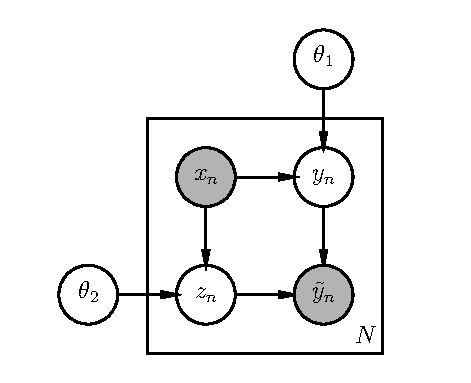
\includegraphics[width=0.5\linewidth]{figure/pgm.pdf}
\end{center}
\caption{Probabilistic graphical model of label noise}
\label{fig:noise_pgm}
\end{figure}

Despite the observed image $\vec{x}$ and the noisy label $\tilde{\vec{y}}$, we exploit two discrete latent variables --- $\vec{y}$ and $\vec{z}$ --- to represent the ground truth and the type of label noise, respectively. Both $\tilde{\vec{y}}$ and $\vec{y}$ are $L$-dimensional binary random variables in 1-of-$L$ fashion, \ie, only one element is equal to 1 while others are all 0.

On the other hand, the latent variable $\vec{z}$ representing label noise type is also an 1-of-3 binary random variable. We assign three semantic meanings to each possible state of $\vec{z}$:
\begin{enumerate}
    \item The label is noise free, \ie, $\tilde{\vec{y}}$ should be equal to $\vec{y}$
    \item The label suffers from a pure random noise, \ie, $\tilde{\vec{y}}$ can take any possible value other than $\vec{y}$
    \item The label suffers from a confusing noise, \ie, $\tilde{\vec{y}}$ can take several values that are easily confused with $\vec{y}$
\end{enumerate}

Following this assignment rule, we define the conditional probability of the noisy label by
\begin{equation} \label{eq:likelihood}
    p(\tilde{\vec{y}}|\vec{y},\vec{z}) = \begin{cases}
        \mat{I}\vec{y} & \text{if } \vec{z}_1 = 1 \\
        \frac{1}{L-1}(\mat{U} - \mat{I})\vec{y} & \text{if } \vec{z}_2 = 1 \\
        \mat{C}\vec{y} & \text{if } \vec{z}_3 = 1
    \end{cases}
\end{equation}
where $\mat{I}$ is the identity matrix, $\mat{U}$ is the unit matrix (all the elements are one), and $\mat{C}$ is a sparse stochastic matrix with $\mathrm{tr}(\mat{C})=0$ and $\mat{C}_{ij}$ denoting the confusion probability between class $i$ and $j$. Then we can derive from Figure~\ref{fig:noise_pgm} the joint distribution of $\tilde{\vec{y}}, \vec{y}$ and $\vec{z}$ conditioning on $\vec{x}$:
\begin{equation} \label{eq:joint_distribution}
  p(\tilde{\vec{y}}, \vec{y}, \vec{z} | \vec{x}) = p(\tilde{\vec{y}} | \vec{y}, \vec{z}) p(\vec{y} | \vec{x}) p(\vec{z} | \vec{x})
\end{equation}

While the object class probability distribution $p(\vec{y} | \vec{x})$ is comprehensible, the semantic meaning of $p(\vec{z} | \vec{x})$ needs extra clarification: it can be seen as a property of an image, which represents how confusing the image is. Specific to our clothes classification problem, $p(\vec{z} | \vec{x})$ can be affected by different factors, including background clutter, image resolution, the style and material of the clothes, \etc. See Figure~\ref{fig:compare_noise_level} for some examples.

\begin{figure}[t]
\begin{center}
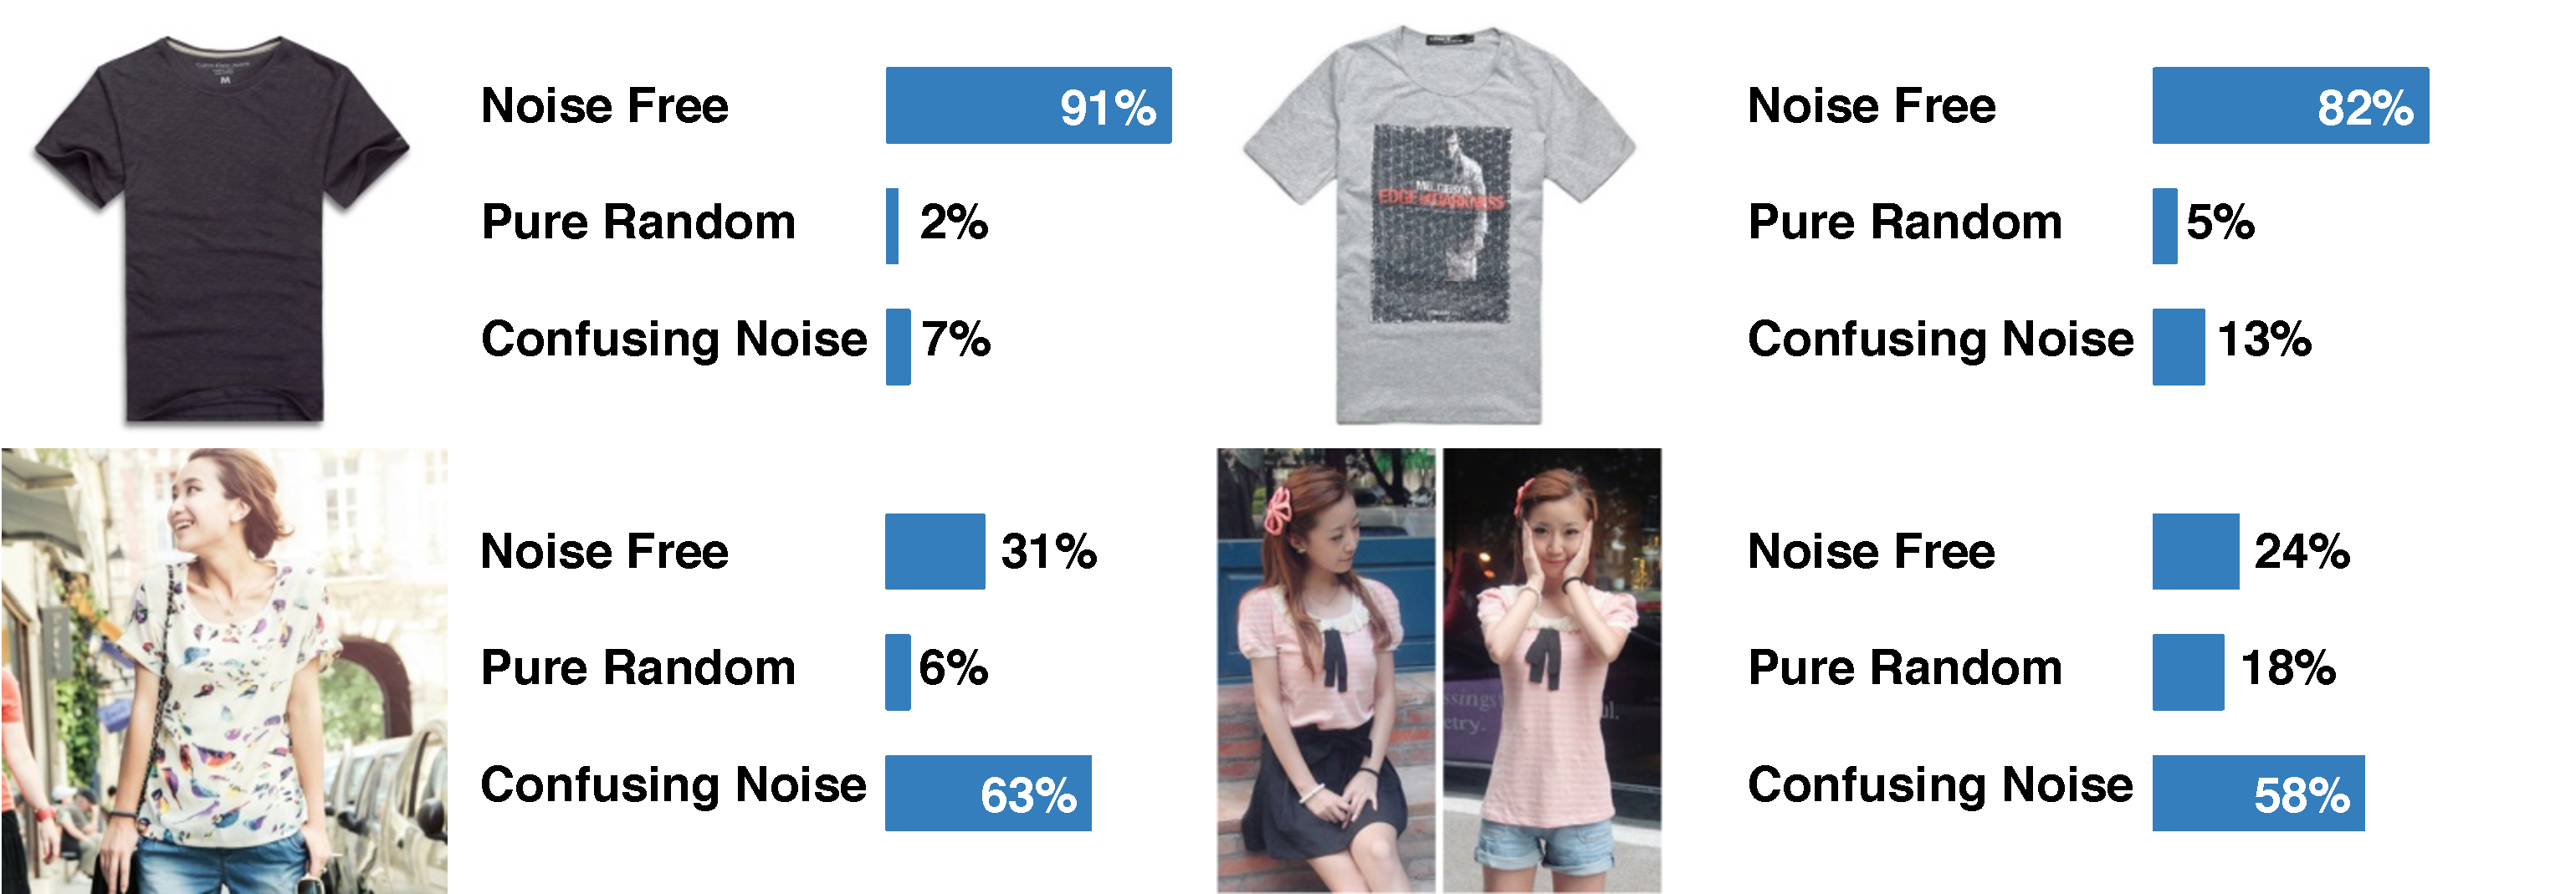
\includegraphics[width=1.0\linewidth]{figure/noise_level.pdf}
\end{center}
\caption{The probability of an image suffering from different noise types depend on the image itself. Although all the images belong to class ``T-shirt'', the top two images can be easily recognized, while the bottom two tend to be confused with class ``Chiffon''.}
\label{fig:compare_noise_level}
\end{figure}

To illustrate the relations between noisy label and ground truth, we can derive their conditional probability from Eq~\ref{eq:joint_distribution} by
\begin{equation}
    p(\tilde{\vec{y}} | \vec{y}, \vec{x}) = \sum_{\vec{z}} p(\tilde{\vec{y}}, \vec{z} | \vec{y}, \vec{x}) = \sum_{\vec{z}} p(\tilde{\vec{y}} | \vec{y}, \vec{z}) p(\vec{z} | \vec{x})
\end{equation}
which can be interpreted as a mixture model. Given an input image $\vec{x}$, the conditional probability $p(\vec{z} | \vec{x})$ can be seen as the prior of each mixture component. This makes a key difference between our work and~\cite{sukhbaatar2014learning}, where they assume $\tilde{\vec{y}}$ is conditionally independent with $\vec{x}$ if $\vec{y}$ is given. All the images share a same noise model in~\cite{sukhbaatar2014learning}, while in our approach each data sample has its own.

\subsection{Learning the Parameters} % (fold)
\label{sub:learning_the_parameters}
We exploit two deep neural networks to model $p(\vec{y} | \vec{x})$ and $p(\vec{z} | \vec{x})$ separately. Denote the parameter set of each deep model by $\theta_1$ and $\theta_2$. Our goal is to find the optimal $\theta = \theta_1 \cup \theta_2$ that maximize the incomplete log-likelihood $\log p(\tilde{\vec{y}} | \vec{x}; \theta)$. Expectation-Maximization algorithm is used to solve this problem iteratively.

For any probability distribution $q(\vec{y}, \vec{z} | \tilde{\vec{y}}, \vec{x})$, we can derive a lower bound of the incomplete log-likelihood by
\begin{equation}
\begin{aligned}
    \log p(\tilde{\vec{y}} | \vec{x}; \theta) &= \log \sum_{\vec{y},\vec{z}} p(\tilde{\vec{y}}, \vec{y}, \vec{z} | \vec{x}; \theta) \\
    &\geq \sum_{\vec{y},\vec{z}} q(\vec{y}, \vec{z} | \tilde{\vec{y}}, \vec{x}) \log \frac{p(\tilde{\vec{y}}, \vec{y}, \vec{z} | \vec{x}; \theta)}{q(\vec{y}, \vec{z} | \tilde{\vec{y}}, \vec{x})}
\end{aligned}
\end{equation}
\textbf{E-Step} The difference between $\log p(\tilde{\vec{y}} | \vec{x}; \theta)$ and its lower bound is the Kullback-Leibler divergence $\mathrm{KL}\left(q(\vec{y}, \vec{z} | \tilde{\vec{y}}, \vec{x}) || p(\vec{y}, \vec{z} | \tilde{\vec{y}}, \vec{x}; \theta)\right)$, which is equal to zero if and only if $q(\vec{y}, \vec{z} | \tilde{\vec{y}}, \vec{x}) = p(\vec{y}, \vec{z} | \tilde{\vec{y}}, \vec{x}; \theta)$. Therefore, in each iteration $t$ of the E-Step, we first compute the posterior of latent variables using current parameters $\theta^{(t)}$:
\begin{multline} \label{eq:posterior}
    p(\vec{y}, \vec{z} | \tilde{\vec{y}}, \vec{x}; \theta^{(t)}) = \frac{p(\tilde{\vec{y}}, \vec{y}, \vec{z} | \vec{x}; \theta^{(t)})}{p(\tilde{\vec{y}} | \vec{x}; \theta^{(t)})} \\
    = \frac{p(\tilde{\vec{y}}|\vec{y},\vec{z};\theta^{(t)}) p(\vec{y}|\vec{x};\theta^{(t)}) p(\vec{z}|\vec{x};\theta^{(t)})}{\sum_{\vec{y}',\vec{z}'} p(\tilde{\vec{y}}|\vec{y}',\vec{z}';\theta^{(t)}) p(\vec{y}'|\vec{x};\theta^{(t)}) p(\vec{z}'|\vec{x};\theta^{(t)})}
\end{multline}
Then the expected complete log-likelihood can be written as
\begin{equation}
    Q(\theta; \theta^{(t)}) = \sum_{\vec{y},\vec{z}} p(\vec{y}, \vec{z} | \tilde{\vec{y}}, \vec{x}; \theta^{(t)}) \log p(\tilde{\vec{y}}, \vec{y}, \vec{z} | \vec{x}; \theta)
\end{equation}
\textbf{M-Step} Since deep neural networks are exploited to model the probability $p(\vec{y}|\vec{x};\theta_1)$ and $p(\vec{z}|\vec{x};\theta_2)$, we perform gradient ascent on $Q$:
\begin{multline} \label{eq:gradient}
    \frac{\partial Q}{\partial \theta} = \sum_{\vec{y},\vec{z}} p(\vec{y}, \vec{z} | \tilde{\vec{y}}, \vec{x}; \theta^{(t)}) \frac{\partial}{\partial \theta} \log p(\tilde{\vec{y}}, \vec{y}, \vec{z} | \vec{x}; \theta) \\
    = \sum_{\vec{y}} p(\vec{y} | \tilde{\vec{y}}, \vec{x}; \theta^{(t)}) \frac{\partial}{\partial \theta_1} \log p(\vec{y}|\vec{x};\theta_1) + \\
      \sum_{\vec{z}} p(\vec{z} | \tilde{\vec{y}}, \vec{x}; \theta^{(t)}) \frac{\partial}{\partial \theta_2} \log p(\vec{z}|\vec{x};\theta_2)
\end{multline}

The M-Step above is equivalent to minimize the cross entropy between the estimated ground truth distribution and the prediction of the classifier.
% subsection learning_the_parameters (end)

\subsection{Estimating the Matrix $\mat{C}$} % (fold)
\label{sub:confusion_estimation}
Notice that we do not set parameters to the conditional probability $p(\tilde{\vec{y}}|\vec{y},\vec{z})$ in Eq~\eqref{eq:likelihood} and keep it unchanged during the learning process. Because without other regularizations, learning all the three parts could lead to trivial solutions. For example, the network will always predict $\vec{y}_1 = 1$, $\vec{z}_3 = 1$, and the matrix $\mat{C}$ is learned to make $\mat{C}_{1i} = 1$ for all $i$. To avoid this degeneration, we choose to give $\mat{C}$ a good estimation while let the deep model learn to predict $p(\vec{y} | \vec{x})$ and $p(\vec{z} | \vec{x})$ for each input image.

We estimate $\mat{C}$ on a relatively small dataset $\mathcal{D}_c = \{(\vec{x},\vec{y},\tilde{\vec{y}})\}_N$, where we have $N$ images with both clean and noisy label. As prior information about $\vec{z}$ is not available, we just solve the following optimization problem:
\begin{equation}
    \max_{\mat{C},\vec{z}^{(1)},\cdots,\vec{z}^{(N)}} \sum_{i=1}^N \log p(\tilde{\vec{y}}^{(i)}|\vec{y}^{(i)},\vec{z}^{(i)})
\end{equation}
Obviously, sample $i$ contributes nothing to the optimal $\mat{C}^*$ if $\vec{y}^{(i)}$ and $\tilde{\vec{y}}^{(i)}$ are equal. So that we ignore those samples and reinterpret the problem in another form by exploiting Eq~\ref{eq:likelihood}:
\begin{equation}
\begin{aligned}
\max_{\mat{C},\vec{t}} \quad & E=\sum_{i=1}^{N'} \log \alpha^{\vec{t}_i} + \log (\tilde{\vec{y}}^{(i)T} \mat{C} \vec{y}^{(i)})^{1-\vec{t}_i}\\
\text{subject to} \quad & \mat{C} \text{ is a stochastic matrix of size } L\times L \\
                    & \vec{t} \in \{0,1\}^{N'}
\end{aligned}
\end{equation}
where $\alpha=\frac{1}{L-1}$ and $N'$ is the number of remaining samples. The semantic meaning of the above formulation is that we need to assign each $(\vec{y},\tilde{\vec{y}})$ pair the optimal noise type, while finding the optimal $\mat{C}$ simultaneously.

Next, we will show that the problem can be solved by a simple yet efficient algorithm in $O(N'+L^2)$ time complexity. Before we introduce the algorithm itself, some theorems need to be proved. Denote the optimal solution by $\mat{C}^*$ and $\vec{t}^*$
\begin{lemma}
$\mat{C}^*_{ij} \neq 0 \Rightarrow \mat{C}^*_{ij} > \alpha, \forall i,j \in \{1,\dots,L\}$
\end{lemma}
\begin{proof}
Suppose there exists some $i,j$ such that $0 < \mat{C}^*_{ij} \leq \alpha$. Then we conduct following operations. First, we set $\mat{C}^*_{ij}=0$ while adding its original value to other elements in column $j$. Second, for all the samples $n$ where $\tilde{\vec{y}}^{(n)}_i=1$ and $\vec{y}^{(n)}_j=1$, we set $\vec{t}_n$ to 1. The resulting $E$ is always greater than the original one, which leads to a contradiction.
\end{proof}
\begin{theorem}
$(\tilde{\vec{y}}^{(i)},\vec{y}^{(i)})=(\tilde{\vec{y}}^{(j)},\vec{y}^{(j)}) \Rightarrow \vec{t}^*_i=\vec{t}^*_j, \forall i,j \in \{1,\dots,N'\}$
\end{theorem}
\begin{proof}
Suppose $\tilde{\vec{y}}^{(i)}_k=\tilde{\vec{y}}^{(j)}_k=1$ and $\vec{y}^{(i)}_l=\vec{y}^{(j)}_l=1$ but $\vec{t}^*_i \neq \vec{t}^*_j$. From Lemma 1 we know that elements in $\mat{C}^*$ is either 0 or greater than $\alpha$. If $\mat{C}^*_{kl}=0$, we can set $\vec{t}^*_i=\vec{t}^*_j=1$, otherwise we can set $\vec{t}^*_i=\vec{t}^*_j=0$. In either case the objective function $E$ is greater than the original one, which draws a contradiction.
\end{proof}
\begin{theorem}
$\tilde{\vec{y}}^{(i)T} \mat{C}^* \vec{y}^{(i)} > \alpha \Leftrightarrow \vec{t}^*_i=0$ and $\tilde{\vec{y}}^{(i)T} \mat{C}^* \vec{y}^{(i)} = 0 \Leftrightarrow \vec{t}^*_i=1, \forall i \in \{1,\dots,N'\}$
\end{theorem}
\begin{proof}
The first part is straight forward. For the second part, $\vec{t}^*_i=1$ implies $\tilde{\vec{y}}^{(i)T} \mat{C}^* \vec{y}^{(i)} \leq \alpha$. By using Lemma 1 we know that $\tilde{\vec{y}}^{(i)T} \mat{C}^* \vec{y}^{(i)} = 0$.
\end{proof}

Notice that if the true label of an image is class $i$ while the noisy label is class $j$, then it can only affect the value of $\mat{C}_{ij}$. Thus each column of $\mat{C}$ can be optimized separately. Theorem 1 further shows that samples with same pair of $(\tilde{\vec{y}},\vec{y})$ share a same noise type. Then what really matters is the frequency of each of the $L\times L$ pairs $(\tilde{\vec{y}},\vec{y})$. Considering a particular column $\vec{c}$, suppose there are $M$ samples affecting this column. We can count the frequency of noisy label class 1 to $L$ as $m_1,\dots,m_L$ and might as well set $m_1\geq m_2\geq \cdots \geq m_L$. The problem is then converted to
\begin{equation}
\begin{aligned}
\max_{\vec{c},\vec{t}} \quad & E=\sum_{k=1}^{L} m_k \left(\log \alpha^{\vec{t}_k} + \log \mat{c}_k^{1-\vec{t}_k}\right)\\
\text{subject to} \quad & \vec{c} \in [0,1]^L, \sum_{k=1}^{L} \vec{c}_k = 1 \\
                    & \vec{t} \in \{0,1\}^{L}
\end{aligned}
\end{equation}

Due to the rearrangement inequality, we can prove that in the optimal solution,
\begin{equation}
    \max(\alpha,\vec{c}^*_1) \geq \max(\alpha,\vec{c}^*_2) \geq \cdots \geq \max(\alpha,\vec{c}^*_L)
\end{equation}
Then by using Theorem 2, there must exist a $k^* \in \{1,\dots,L\}$ such that
\begin{equation} \label{eq:opt_t}
\begin{aligned}
    &\vec{t}^*_i = 0, i = 1,\dots,k^* \\
    &\vec{t}^*_i = 1, i = k^*+1,\dots,L
\end{aligned}
\end{equation}
This also implies that only the first $k^*$ elements of $\vec{c}^*$ have nonzero values (greater than $\alpha$ actually). Furthermore, if $k^*$ is known, finding the optimal $\vec{c}^*$ is to solve the following problem:
\begin{equation}
\begin{aligned}
\max_{\vec{c}} \quad & E=\sum_{k=1}^{k^*} m_k \log \mat{c}_k\\
\text{subject to} \quad & \vec{c} \in [0,1]^L, \sum_{k=1}^{k^*} \vec{c}_k = 1
\end{aligned}
\end{equation}
whose solution is
\begin{equation} \label{eq:opt_c}
\begin{aligned}
    &\vec{c}^*_i = \frac{m_i}{\sum_{k=1}^{k^*}{m_k}}, i = 1,\dots,k^* \\
    &\vec{c}^*_i = 0, i = k^*+1,\dots,L
\end{aligned}
\end{equation}

The above analysis leads to a simple algorithm. We enumerate $k^*$ from 1 to $L$. For each $k^*$, $\vec{t}^*$ and $\vec{c}^*$ are computed by using Eq~\eqref{eq:opt_t} and~\eqref{eq:opt_c}, respectively. Then we evaluate the objective function $E$ and record the best solution.


% subsection confusion_estimation (end)

% section label_noise_model (end)

\section{Deep Learning from Noisy Labels} % (fold)
\label{sec:weak_label_deep_learning}

\begin{figure*}
\begin{center}
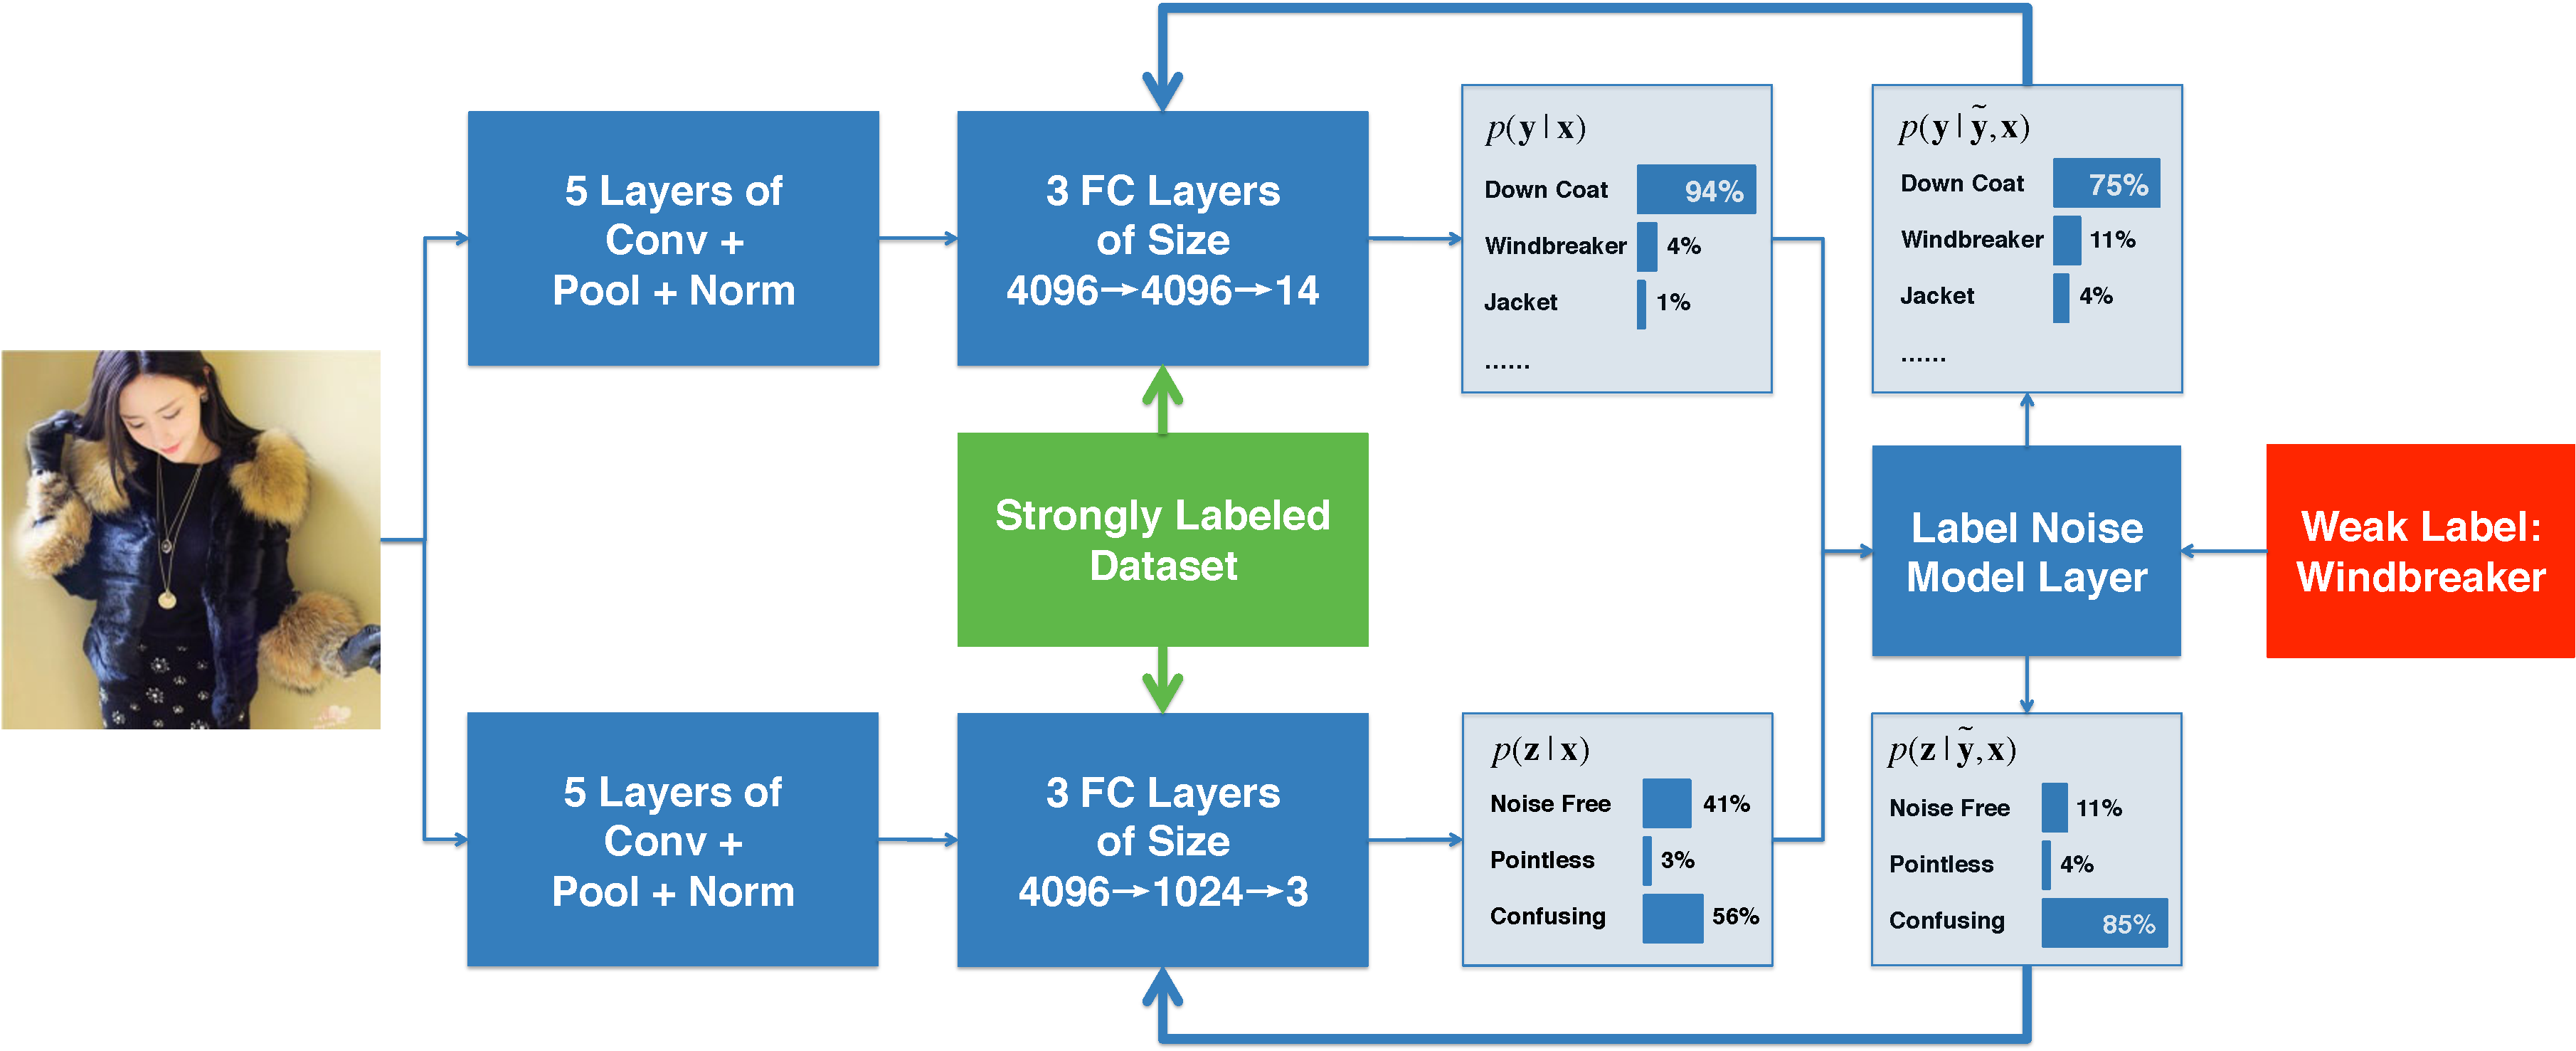
\includegraphics[width=0.9\linewidth]{figure/diagram.pdf}
\end{center}
\caption{System diagram of our proposed method. Two CNNs are exploited to predict object class $p(\vec{y}|\vec{x})$ and noise type $p(\vec{z}|\vec{x})$ respectively. A label noise model layer infers the ground truths according to CNNs' results and the observed noisy label. The ground truth is then used to supervise the CNNs. A separate strongly labeled dataset is also utilized to prevent the model from drifting away.}
\label{fig:framework}
\end{figure*}

We integrate the proposed label noise model into a deep learning framework. As demonstrated in Figure~\ref{fig:framework}, we predict the probability $p(\vec{y}|\vec{x})$ and $p(\vec{z}|\vec{x})$ by using two independent CNNs. Moreover, we append a label-noise-model layer at the end, which takes as input the CNNs' prediction scores and the observed noisy label. Stochastic Gradient Ascent (SGA) with backpropagation technique is used to approximately optimize the whole network. In each forward pass, the label-noise-model layer computes the posterior of latent variables according to Eq~\eqref{eq:posterior}. While in the backward pass, it computes the gradients according to Eq~\eqref{eq:gradient}.

% The forward procedure is summarized in Algorithm~\ref{alg:forward}, and the backward pass for computing gradient with respect to $p(\vec{y}|\vec{x})$ is illustrated in Algorithm~\ref{alg:backward}.

% \begin{algorithm}
%     \SetKwData{Sum}{sum}
%     \SetKwFunction{Softmax}{Softmax}\SetKwFunction{Q}{Q}
%     \SetKwInOut{Input}{input}\SetKwInOut{Output}{output}

%     \Input{Observed weak label vector $\tilde{\vec{y}}$ of size $N$}
%     \Input{Object class scores matrix $Y$ of size $N \times L$}
%     \Input{Noise type scores matrix $Z$ of size $N \times 3$}
%     \Output{Posterior probability matrix $P$ of size $L \times 3$}
%     \BlankLine

%     $P_y \leftarrow$ \Softmax{$Y$}\;
%     $P_z \leftarrow$ \Softmax{$Z$}\;
%     \BlankLine

%     \emph{\Q is the function that implements Eq~\eqref{eq:likelihood}}\;
%     \BlankLine

%     \For {$i \leftarrow 1$ \KwTo $N$} {
%         \Sum $\leftarrow 0$\;
%         \For {$j \leftarrow 1$ \KwTo $L$} {
%             \For {$k \leftarrow 1$ \KwTo $3$} {
%                 $P[i,j,k] \leftarrow P_y[i,j] \times P_z[i,k] \times$ \Q{$\tilde{\vec{y}}$,j,k}\;
%                 \Sum $\leftarrow$ \Sum$+ P[i,j,k]$\;
%             }
%         }
%         $P[i,:,:] \leftarrow P[i,:,:] /$ \Sum\;
%     }

%     \caption{Forward pass}
%     \label{alg:forward}
% \end{algorithm}
% \begin{algorithm}
%     \SetKwData{Sum}{sum}
%     \SetKwInOut{Input}{input}\SetKwInOut{Output}{output}

%     \Input{Object class scores matrix $Y$ of size $N \times L$}
%     \Input{Posterior probability matrix $P$ of size $L \times 3$}
%     \Output{Gradient matrix $\Delta_Y$ of size $N \times L$}
%     \BlankLine

%     \For {$i \leftarrow 1$ \KwTo $N$} {
%         \For {$j \leftarrow 1$ \KwTo $L$} {
%             \Sum $\leftarrow 0$\;
%             \For {$k \leftarrow 1$ \KwTo $3$} {
%                 \Sum $\leftarrow$ \Sum$+ P[i,j,k]$\;
%             }
%             $\Delta_Y[i,:] \leftarrow \Delta_Y[i,:] + $ \Sum $\times Y[i,:]$\;
%             $\Delta_Y[i,j] \leftarrow \Delta_Y[i,j] - $ \Sum\;
%         }
%     }


%     \caption{Backward pass for computing gradient w.r.t. object class scores}
%     \label{alg:backward}
% \end{algorithm}

Directly training the whole network with random initialization is impractical, because the posterior computation could be totally wrong. Therefore, we need to pretrain each CNN component with strongly supervised data. Gathering ground truth object classes is straight forward, since we can just manually label some images by expert. The resulting strongly labeled dataset $\mathcal{D}_c$ can be directly used for training the network that predicts $p(\vec{y}|\vec{x})$. On the other hand, although off-the-shelf supervision for $p(\vec{z}|\vec{x})$ is not available, we can heuristically generate some data by utilizing the images having both strong and noisy labels. For each sample, we choose as ground truth the $\vec{z}$ that maximizes the likelihood in Eq~\eqref{eq:likelihood}.

After both the CNN components are properly pretrained, we can start training the whole network with massive noisy labeled data. However, some practical issues need to be further discussed. First, if we merely use noisy labels, we will lose precious knowledge that we have gained before and the model could be drifted. Therefore, we need to mix strongly label data together in to our training set, which is depicted in Figure~\ref{fig:framework} as the extra supervisions for the two CNN components. Then each CNN receives two kinds of gradients, one is from the clean labeled data and the other is from the noisy labeled data. We denote them by $\Delta_c$ and $\Delta_n$, respectively. A potential problem is that $|\Delta_c| \ll |\Delta_n|$, because clean data is much less than the noisy data. To deal with this problem, we bootstrap the clean data $\mathcal{D}_c$ to half amount of the noisy data $\mathcal{D}_n$. This upsampling process brings another advantage --- the gradients we calculated in each mini-batch are much more stable.

Our proposed method has the ability to figure out the ground truth label given the image and its noisy label. From the perspective of information, our model predicts from two kinds of clues: what are the true labels for other similar images; and how confusing is the input image itself. Label Propagation method~\cite{zhu2002learning} explicitly uses the first kind of information, while we implicitly capture it with a discriminative deep model. Meanwhile, we exploit the second kind of information to bridge the semantic gap between the image and its possible noisy labels.
% section weak_label_deep_learning (end)

\section{Experiments} % (fold)
\label{sec:experiments}

\subsection{Dataset} % (fold)
\label{sub:dataset}
We build a large-scale clothes dataset by crawling images and their surrounding texts from some online shopping websites. These surrounding texts are valuable, because they usually contain several keywords that can be further converted to visual tags. Specific to our task of clothes classification, we define $14$ classes: T-shirt, Shirt, Knitwear, Chiffon, Sweater, Coat, Windbreaker, Jacket, Down Coat, Suit, Shawl, Dress, Vest, and Underwear.

In order to learn a clothes classifier and evaluate its performance, we manually label a small part of all the images and split it into training ($\mathcal{D}_c$), validation and test sets. Meanwhile the remaining data construct the noisy labeled training dataset $\mathcal{D}_n$. A crucial data preprocessing step is to remove near duplicate images from $\mathcal{D}_c$ and $\mathcal{D}_n$, which ensures the reliability of our test protocol. The size of training datasets are $|\mathcal{D}_c| = 47570$ and $|\mathcal{D}_n| = 1.5M$, while validation and test set consist of 14,313 and 10,526 images respectively. The confusion matrix between clean and noisy labels are presented in Figure~\ref{fig:cm_strong_weak}. We can see that the overall accuracy is only $61.54\%$, which means that the labels converted from surrounding texts are quite noisy.

\begin{figure}[t]
\begin{center}
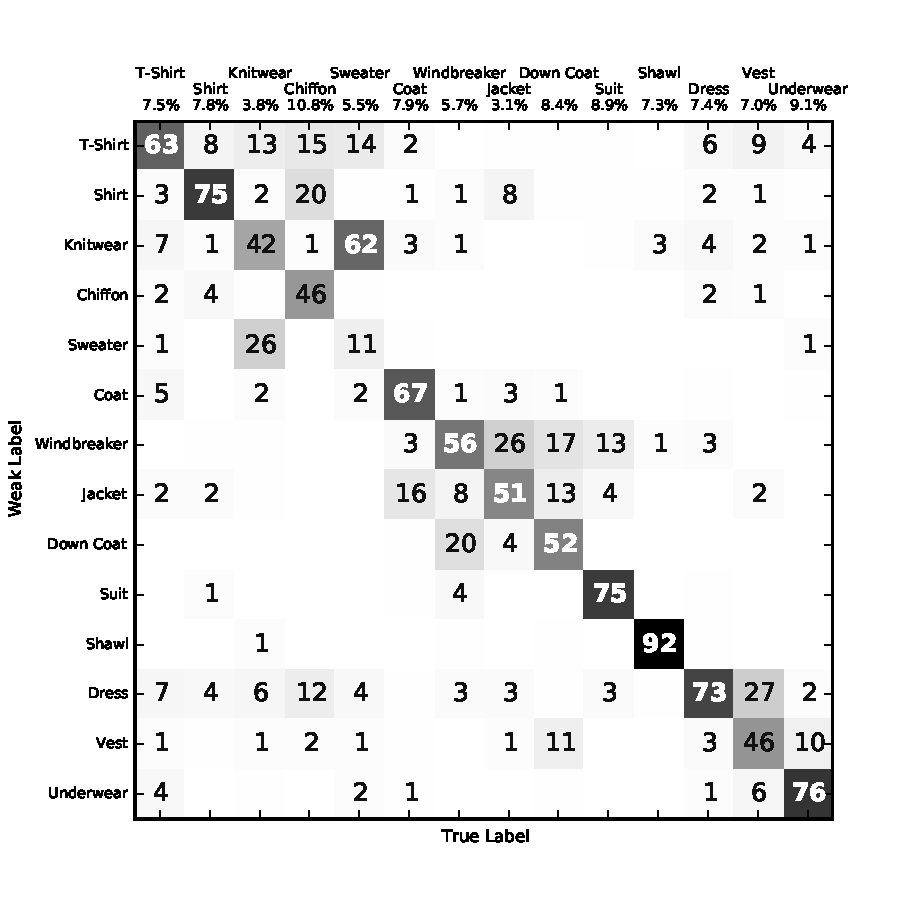
\includegraphics[width=1.0\linewidth]{figure/cm_strong_weak_labels.pdf}
\end{center}
\caption{\textbf{Confusion matrix between clean and noisy labels}. We hide extremely small grid numbers for better demonstration. Frequency of each true label is listed at the top of each column. The overall accuracy is $61.54\%$, which indicates that the noisy labels are not reliable.}
\label{fig:cm_strong_weak}
\end{figure}

% subsection dataset (end)

\subsection{Evaluation} % (fold)
\label{sub:evaluation}
The effectiveness of our model is validated based on a series of experiments. We exploit the AlexNet~\cite{krizhevsky2012imagenet} as our baseline model, which consists of five convolutional layers and three fully connected layers. Although recent models may have better learning capability, we choose AlexNet since it is well studied and much easier to be reimplemented (see the \texttt{bvlc\_reference\_caffenet}\footnote{\url{http://caffe.berkeleyvision.org/model_zoo.html}}).

We also implement the bottom up method introduced in~\cite{sukhbaatar2014learning}. Briefly speaking, they proposed a noise model with the assumption that a noisy label is only related to its true label. The relation is built by a confusion matrix $Q$ whose values can be easily obtained as Figure~\ref{fig:cm_strong_weak} in our problem.

We list all the models and training strategies to be compared in Table~\ref{tab:models}.  In general, we set the initial learning rate to be $0.001$ and is multiplied by $0.1$ every $50000$ iterations. For each method, we keep training the model until it converges. Classification accuracies on both the validation and test set are presented in Table~\ref{tab:accuracy}.

\begin{table}
\begin{center}
\begin{tabular}{c|p{3.5em}|p{8em}|p{6em}}
\hline
\# & Method & Data & Initialization \\
\hline\hline
1 & AlexNet & $\mathcal{D}_c$ & random \\
\hline
2 & AlexNet & $\mathcal{D}_c$ & \texttt{ilsvrc2012} pretrained model \\
\hline
3 & AlexNet & $\mathcal{D}_c \cup \mathcal{D}_n$ but treat noisy labels in $\mathcal{D}_n$ as ground truth & random \\
\hline
4 & AlexNet & $\mathcal{D}_c \cup \mathcal{D}_n$ but treat noisy labels in $\mathcal{D}_n$ as ground truth & \texttt{ilsvrc2012} pretrained model \\
\hline
5 & Bottom Up~\cite{sukhbaatar2014learning} & $\mathcal{D}_c \cup \mathcal{D}_n$ & model \#2 \\
\hline
6 & Ours & $\mathcal{D}_c \cup \mathcal{D}_n$ & model \#2 \\
\hline
\end{tabular}
\end{center}
\caption{Models and corresponding training strategies used in our experiments}
\label{tab:models}
\end{table}

\begin{figure*}
\begin{center}
\end{center}
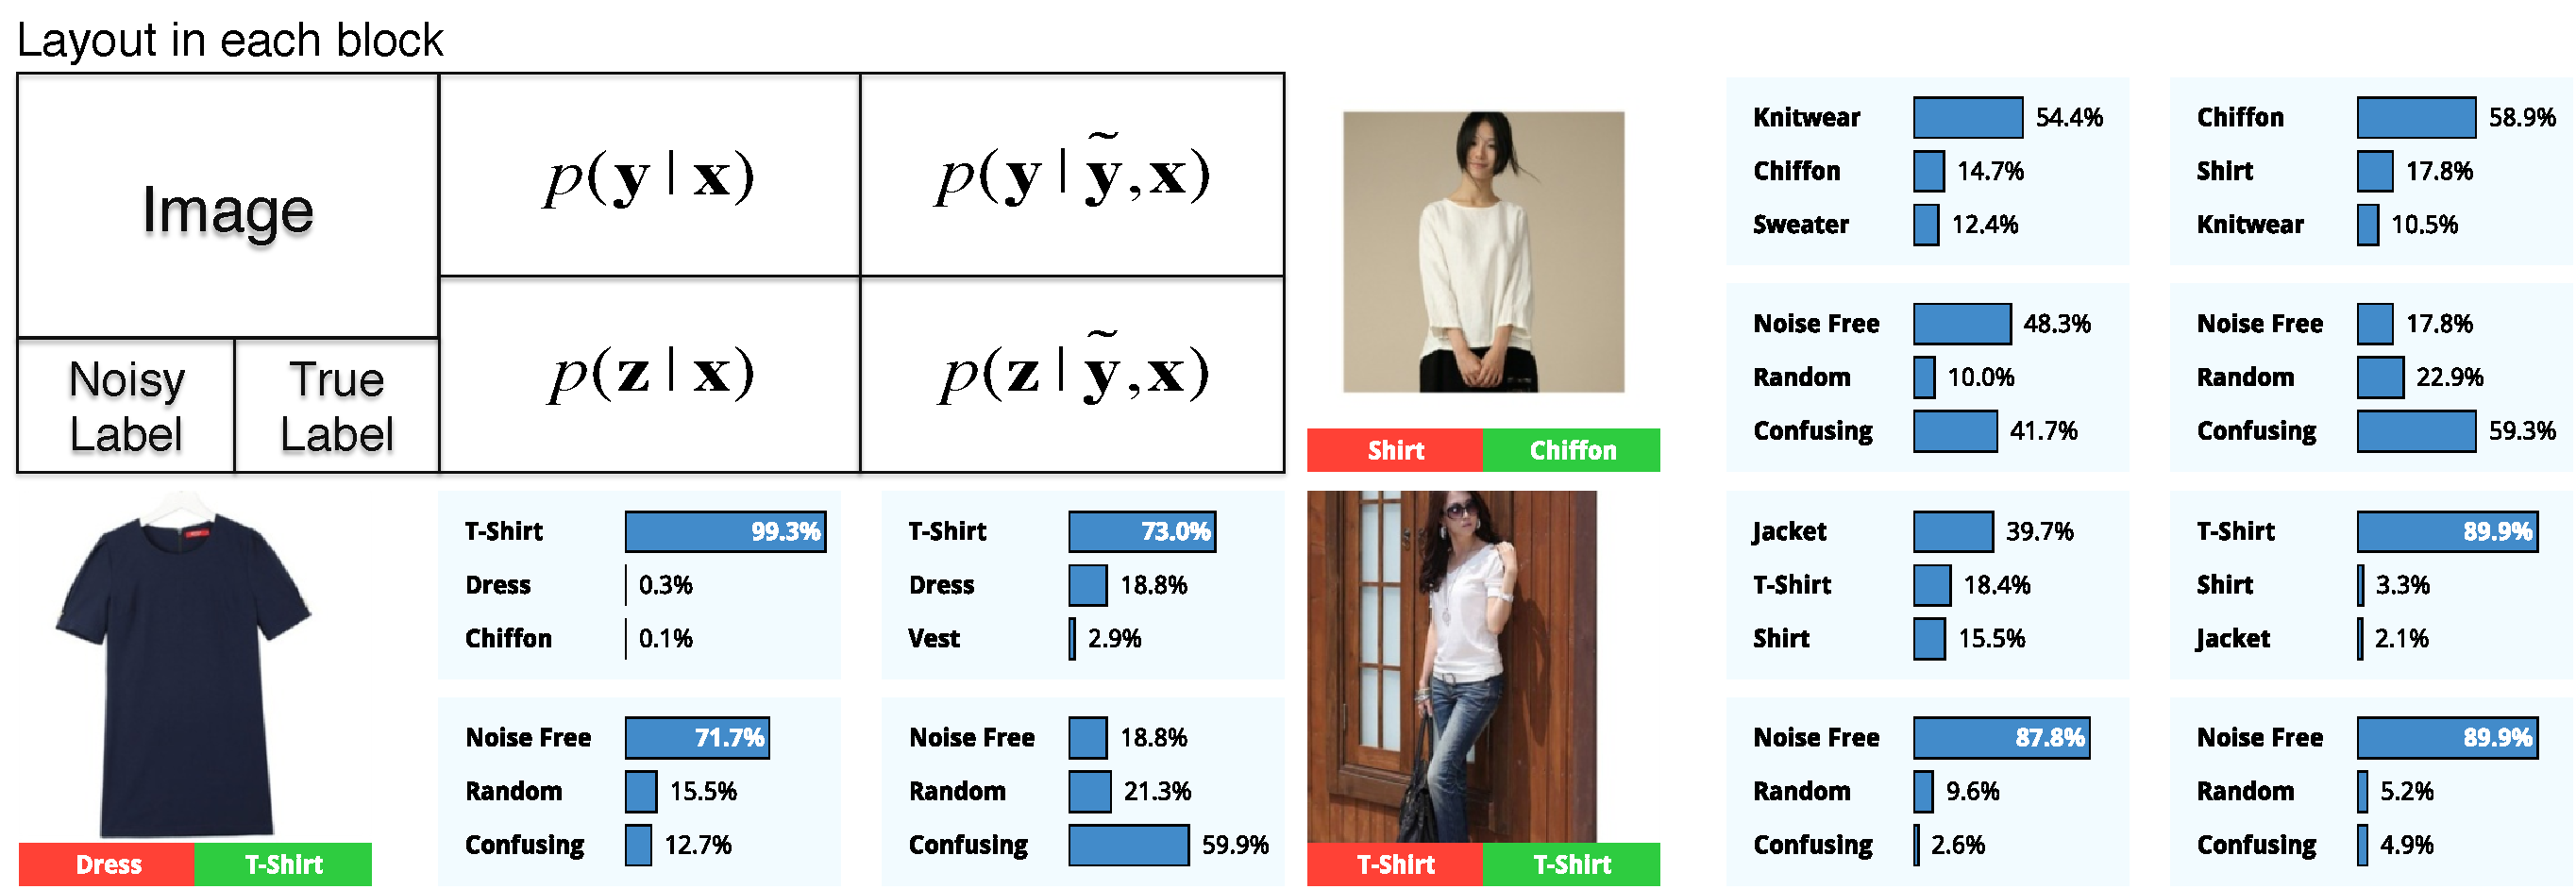
\includegraphics[width=1.0\linewidth]{figure/model_output.pdf}
\caption{\textbf{Examples of model predictions}. The information layout in each block is illustrated in the top-left one.}
\label{fig:model_output}
\end{figure*}

From row 1 we can see that when only a small amount of strongly supervised data is provided to train the deep neural network, the parameters cannot be learned properly and thus results in a bad performance. To cope with this problem, finetuning from a model pretrained on related but much larger dataset can significantly improve the accuracy, which is illustrated in the result of model \#2. This is a commonly used technique to train a deep model with limited data for specific task.

However, this transfer learning scheme may still suffer from suboptimal model parameters if the datasets for pretraining and finetuning are loosely related, just like the clothes vs. general objects in our case. We see from row 3 that better performance can be achieved when we train the same model with random initialization on massive data with label noise, but treat noisy labels just as ground truth. Model \#4 further improves the accuracy by initializing with ImageNet pretrained model.

\begin{table}
\begin{center}
\begin{tabular}{c|c|c}
\hline
\# & Validation Accuracy & Test Accuracy \\
\hline\hline
1 & 64.28\% & 64.54\% \\
\hline
2 & 72.21\% & 72.63\% \\
\hline
3 & 73.76\% & 74.03\% \\
\hline
4 & 75.57\% & 75.30\% \\
\hline
5 & 75.97\% & 76.22\% \\
\hline
6 & 77.65\% & 78.24\% \\
\hline
\end{tabular}
\end{center}
\caption{Classification accuracies on validation and test set}
\label{tab:accuracy}
\end{table}


Row 5 and 6 show the effect of handling label noise. While model \#5 is only $0.4\% \sim 0.9\%$ better than the baseline model \#4, our proposed method gains improvement of $2.1\% \sim 2.9\%$. Since model \#5 assumes that the noisy label only relates to the ground truth, which may not be appropriate in our problem. On the contrary, our model predicts the noise type from the image itself. We will discuss about it in the following section.
% subsection evaluation (end)

\subsection{Effect of Noise Estimation} % (fold)
\label{sub:effect_of_noise_estimation}
In order to understand the way our model handles noisy labels, we demonstrate several examples in Figure~\ref{fig:model_output}. We can see that given a noisy label, our model could exploit its current prediction to correct the noise by setting a large weight to the true label, and then use it as supervision instead of the noisy one. Another interesting observation is that if $p(\vec{y}|\vec{x})$ or $p(\vec{z}|\vec{x})$ goes wrong as shown in the top-right and bottom-left block respectively, our model can still figure out the correct label.

Next we explain the meaning of $p(\vec{z}|\vec{x})$ by taking a look at our model's prediction on samples drawn from the clean label class ``Coat''. As shown in Figure~\ref{fig:noise_cluster}, the noisy label is not simply related to the ground truth. On the contrary, images that have high probability of confusing noise tend to share similar visual patterns. This observation indicates that $p(\vec{z}|\vec{x})$ is a property of an image itself representing how confusing the image is. Our model is trained to capture these information and exploit them to clarify the noisy labels. Figure~\ref{fig:noise_prediction_rp} further shows the rank-precision curve of our model's noise prediction. We can see that nearly $80\%$ of the top-500 high confident ``confusing'' samples actually suffer from noise, which again verifies the feasibility of our proposed noise model.

\begin{figure}[t]
\begin{center}
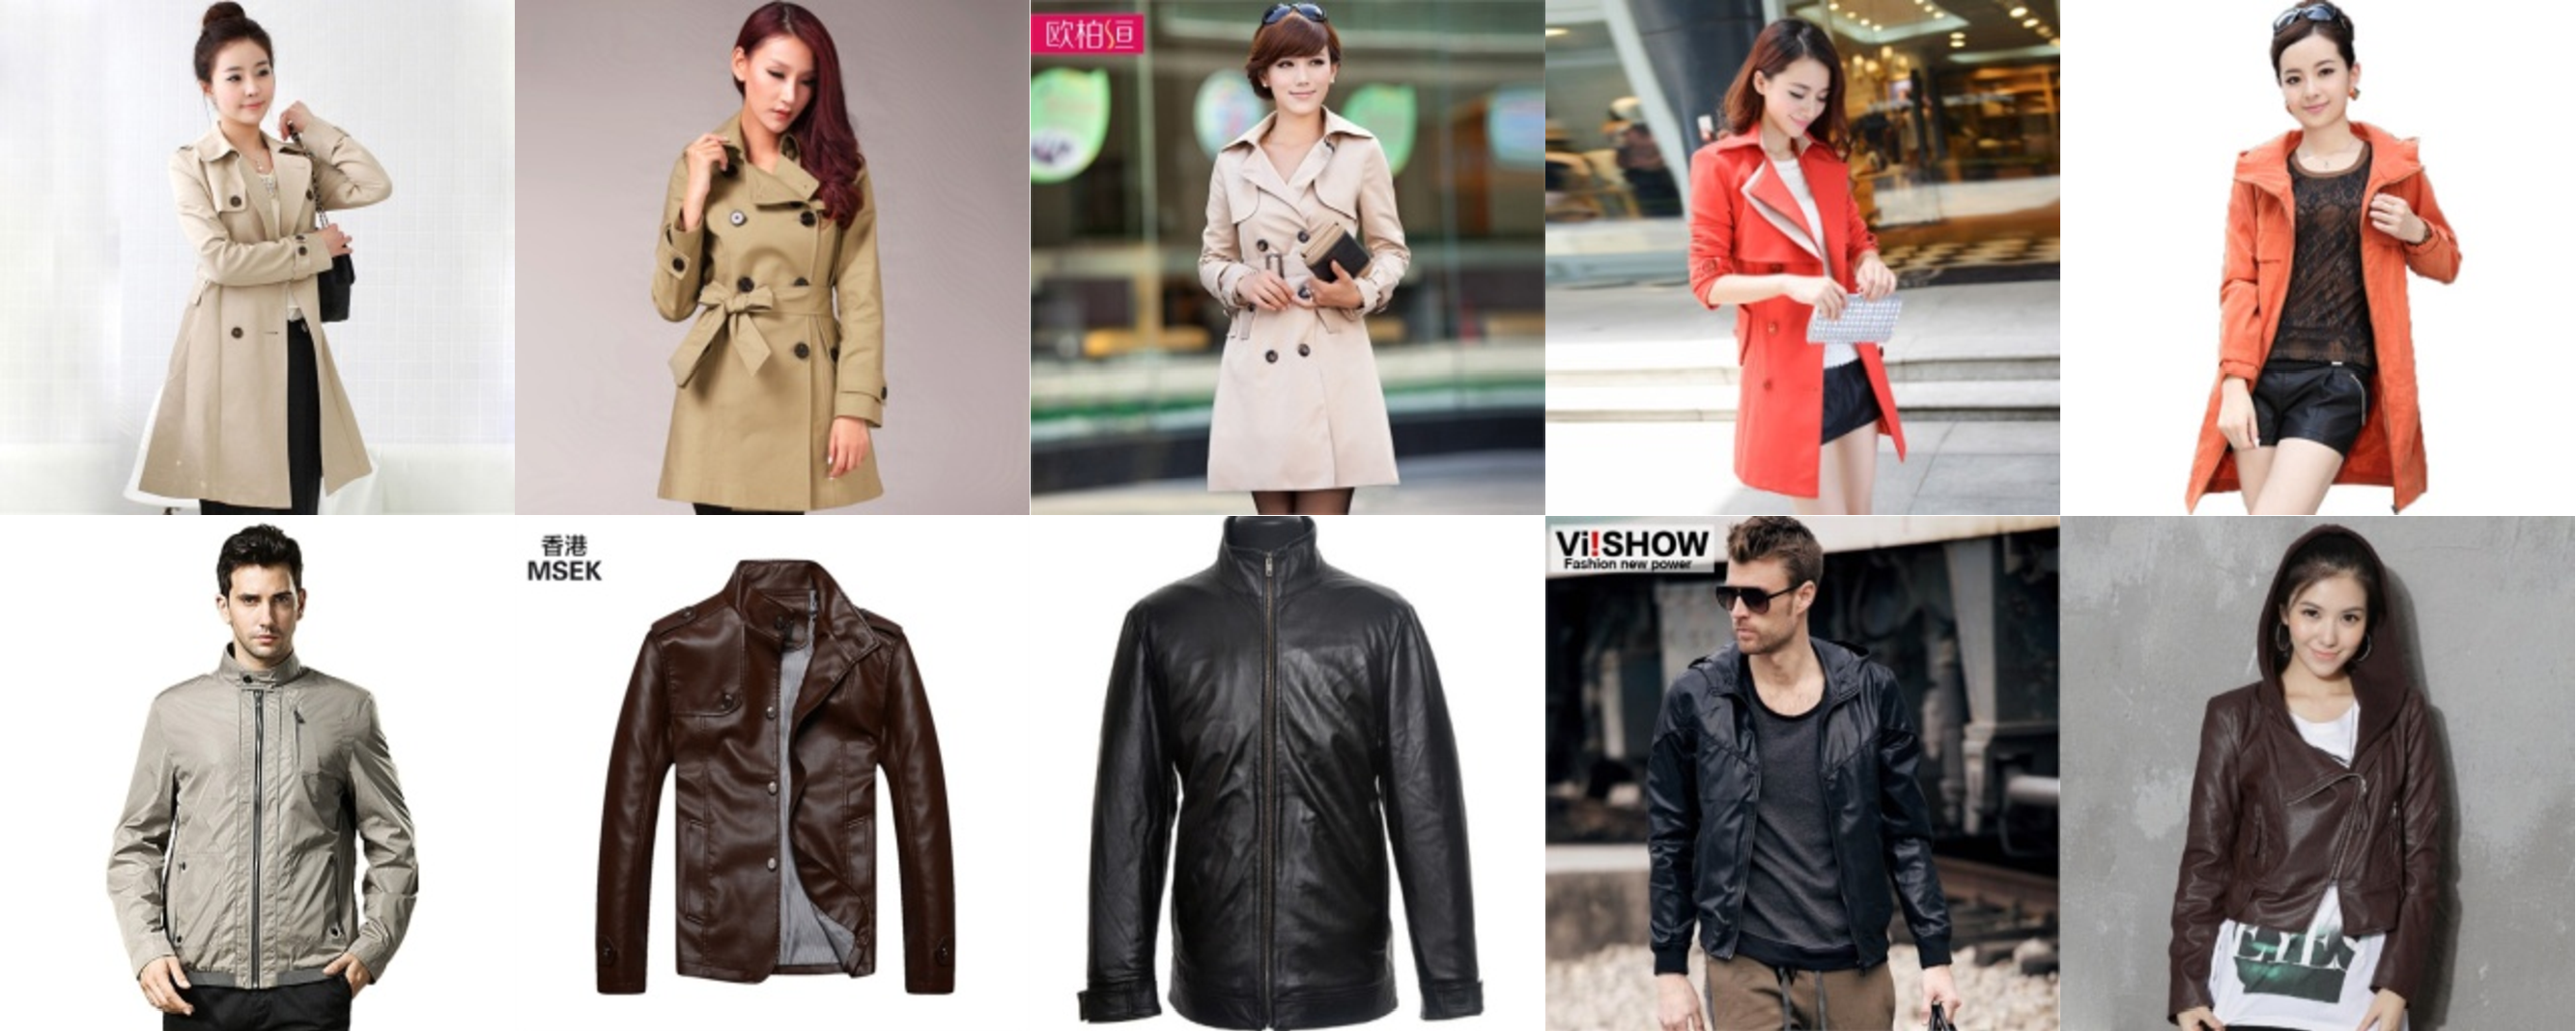
\includegraphics[width=1.0\linewidth]{figure/noise_cluster.pdf}
\end{center}
\caption{Images tend to suffer from confusing noise usually share similar visual patterns. Our model predicts high probability of ``noise free'' for the five images on the top, while predicting high probability of ``confusing noise'' for the bottoms. While all the images share the same clean label ``Coat'', the first three images at the bottom row have noisy label ``Windbreaker'' and the latter two have noisy label ``Jacket''.}
\label{fig:noise_cluster}
\end{figure}

\begin{figure}[t]
\begin{center}
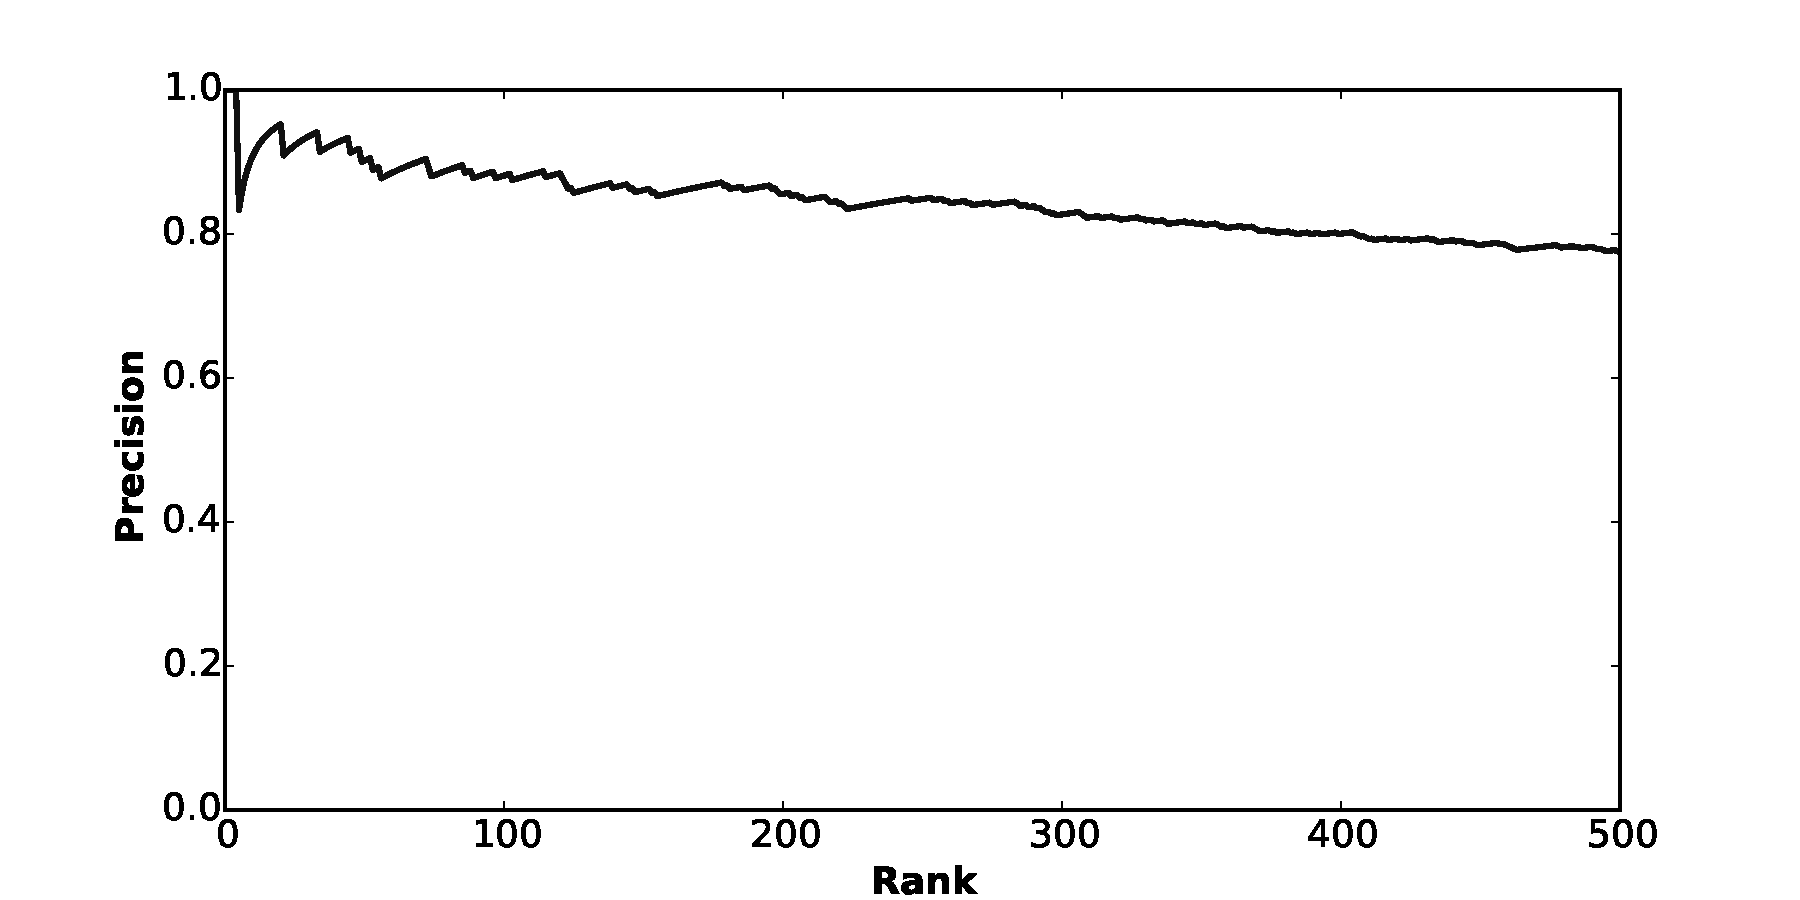
\includegraphics[width=0.8\linewidth]{figure/noise_prediction_rank_precision.pdf}
\end{center}
\caption{We first sort our model's ``confusing noise'' prediction on the validation set, and then check whether the noisy label of the corresponding image mismatch its true label. The rank-precision curve is plotted.}
\label{fig:noise_prediction_rp}
\end{figure}
% subsection effect_of_noise_estimation (end) 
% section experiments (end)

\section{Conclusion} % (fold)
\label{sec:conclusion}
In this paper, we raised the problem of training a deep neural network with limited clean annotations and massive noisy labeled data. A novel end-to-end deep learning framework is proposed to handle label noise in training data. We exploit a novel probabilistic model to describe how a noisy label is generated. Two latent variables --- ground truth and noise type -- are introduced to bridge the semantic gap between the observed image and its corresponding noisy label. We solve the problem by EM algorithm and integrate it into the deep learning framework. Experiments on a large-scale clothes dataset show that massive noisy label data could benefit the training of deep models, and utilizing our noise handling method can further improve the performance.
% section conclusion (end)

\section*{Acknowledgements}
\label{sec:acknowledgements}
This work is supported by the National Basic Research Program of China (973 program No. 2014CB340505).


{\small
\bibliographystyle{ieee}
\bibliography{references}
}

\end{document}
